\documentclass[a4paper,10pt]{article}

% standard packages
\usepackage[utf8]{inputenc}
\usepackage[english]{babel}
\usepackage{csquotes}
\usepackage{geometry}
\usepackage{graphicx}
\usepackage[textsize=footnotesize]{todonotes}

% This is needed for multiple bib-files
% \usepackage[
% 	sortcites=true,
% 	backend=bibtex,
% 	style=ieee,
% 	defernumbers=true,
% ]{biblatex}
% \addbibresource{references.bib} % The name of your bibliography file

% load macros (section title can be changed here)
% section title macros (can be changed)
\newcommand{\insertProjectFundingSchemeTitle}{Project Funding Scheme:}
\newcommand{\insertProjectShortSummaryTitle}{Short Summary:}

% other macros (do not change)
\makeatletter

\newcommand\projectCode[1]{\renewcommand{\insertProjectCode}{#1}}
\newcommand\insertProjectCode{\@latex@error{No \noexpand\projectCode given}\@ehc}

\newcommand\projectTitle[1]{\renewcommand{\insertProjectTitle}{#1}}
\newcommand\insertProjectTitle{\@latex@error{No \noexpand\projectTitle given}\@ehc}

\newcommand\projectPIs[1]{\renewcommand{\insertProjectPIs}{#1}}
\newcommand\insertProjectPIs{\@latex@error{No \noexpand\projectPIs given}\@ehc}

\newcommand\projectFundingScheme[1]{\renewcommand{\insertProjectFundingScheme}{#1}}
\newcommand\insertProjectFundingScheme{\@latex@error{No \noexpand\projectFundingScheme given}\@ehc}

\newcommand\projectShortSummary[1]{\renewcommand{\insertProjectShortSummary}{#1}}
\newcommand\insertProjectShortSummary{\@latex@error{No \noexpand\projectShortSummary given}\@ehc}

%\newcommand\insertProjectHeader{
%  \noindent\hrulefill\\[.5em]
%  \noindent\llap{\fbox{\bfseries\insertProjectCode}\hspace{1em}}{\Large\bfseries\insertProjectTitle} \\[.5em]
%  PIs: \insertProjectPIs\\
%  \null\hrulefill \\[.5em]
%  \begin{tabular}{@{}ll}
%    {\bfseries\insertProjectFundingSchemeTitle} & \insertProjectFundingScheme \\[.5em]
%    {\bfseries\insertProjectShortSummaryTitle} & \insertProjectShortSummary
%  \end{tabular}\\[.5em]
%  \null\hrulefill
%}

\usepackage{tabularx}

\newcommand\insertProjectHeader{
  \noindent\hrulefill\\[.5em]
  \noindent\llap{\fbox{\bfseries\insertProjectCode}\hspace{1em}}{\Large\bfseries\insertProjectTitle} \\[.5em]
  PIs: \insertProjectPIs\\
  \null\hrulefill \\[.5em]
  \begin{tabularx}{\textwidth}{@{} l X @{}}
    {\bfseries\insertProjectFundingSchemeTitle} & \insertProjectFundingScheme \\[.5em]
    {\bfseries\insertProjectShortSummaryTitle} & \insertProjectShortSummary
  \end{tabularx}\\[.5em]
  \null\hrulefill
}

\makeatother



%%%%%%%%%%%%%%%%%%%%%%%%%%%%%%%%%%%%%%%%%%%%%%%%%%%%%%%%%%%%%%%%%%%%%%%%%%%%%%%%
% PLEASE NOTE THE FOLLOWING LENGTH RESTRICTION:
% - no more than 4 pages (incl. publications). 
% - no more than 8 pages (incl. publications) in the exceptional case that you apply for two positions
%%%%%%%%%%%%%%%%%%%%%%%%%%%%%%%%%%%%%%%%%%%%%%%%%%%%%%%%%%%%%%%%%%%%%%%%%%%%%%%%

\newcommand{\bibfilename}{mrabbrev,mybibfile} % <- replace 'mybibfile' with basename of your bibfile


%%%%%%%%%%%%%%%%%%%%%%%%%%%%%%%%%%%%%%%%%%%%%%%%%%%%%%%%%%%%%%%%%%%%%%%%%%%%%%%%
% FILL OUT PROJECT INFORMATION

%%%%% PROJECT CODE
% Please assign your planned project to one Application Area or Emerging Field of MATH+.
% Code "AA1": Application Area 1 (Life Sciences)
% Code "AA2": Application Area 2 (Materials, Light, Devices)
% Code "AA3": Application Area 3 (Networks)
% Code "AA4": Application Area 4 (Energy and Markets)
% Code "EF1": Emerging Field 1 (Extracting Dynamical Laws from Complex Data)
% Code "EF2": Emerging Field 2 (Digital Shapes)
% Code "EF3": Emerging Field 3 (Model-Based Imaging)
% Code "EF4": Emerging Field 4 (Particles and Agents)
% Code "EF5": Emerging Field 5 (Concepts of Change in Historical Processes)
\projectCode{AA2}

%%%%% PROJECT TITLE
% e.g., Deep learning in Berlin administrations
\projectTitle{Multi Material Electocatalysis II}
%%%%% PIs / Applicants
% Project _heads_ only!
% In case a doctoral researcher is to be selected for a position in the project, 
% applicants must indicate with "*" which PI will act as authorized PhD-supervisor. 
% Form: initial dot lastname, initial dot lastname
\projectPIs{J. Fuhrmann, M. Landstorfer}

%%%%% REQUESTED STAFF
% Please use the following code for the position you request:
% Category A)	Full positions (100% E13) for 2 years, 
% Category B)	75% positions (E13) for 3 years (for projects in AAs and EFs only). 
% If you already know whom you intend to hire, please include the name such as "Category A (Dr. Angela Merkel); Start: 1 JAN 2021"
% In this case, please also include the CV of this person as an additional document in your proposal.
\projectFundingScheme{Category A (Dr. Rüdiger Müller); Start: 1 JAN 2021}

%%%%% SHORT SUMMARY
% Please add a short summary of your project using a maximum of 100 words or 5 lines!!!
\projectShortSummary{Here comes the short summary of at most 100 words or 5 lines of text!}

%%%%%%%%%%%%%%%%%%%%%%%%%%%%%%%%%%%%%%%%%%%%%%%%%%%%%%%%%%%%%%%%%%%%%%%%%%%%%%%%
% MAIN CONTENT

\begin{document}

\insertProjectHeader
\todo{JF: Denselben Titel zu haben, ist ggf keine gute Idee}


\subsection*{Extended Synopsis of the Proposal}

\paragraph{Background}
% Please include here:
% use \cite{} to reference publications

% - Account of the problem
% - Motivation
Better theoretical understanding of complex electrocatalytic reactions is
crucial in order to increase the efficiency  and scalability  of electrocatalytic processes
and is therefore a highly relevant topic of research.
The pivotal strategic importance of  technologies based on electrocatalytic reactions
is underlined in  the  recently  approved  National Hydrogen  Strategy of  the  German
Federal  Government. This initiative  grants  hydrogen,  and  in   particular  ``green
hydrogen''  created with  renewable  energy a  strategic  role in  the
decarbonization of the economy as an energy carrier, an energy storage
option, a  sector coupling  technology, a  precursor for  the chemical
industry  and a  means  for  CO2  emission reduction  in  various
industrial  processes. 
As  a part  of this  strategy, the  creation of
hydrogen  from  electrical energy  in  electrolyzers  and the  reverse
process --  the recovery  of electrical energy  from hydrogen  in fuel
cells -- are seen  as indispensable technologies whose development
shall be  supported by  R\&D investments  and market  incentives.
\todo{JF: Die Wasserstoffstrategie ist stark markt- und Technologieorientiert,
  und gibt nicht mehr konkretes zu F\&E her...}
%
Both technologies are based  on electrocatalytic reactions. Production
and utilization  of hydrogen are just  two examples for this  class of
reactions, other  electrocatalytic reactions  are fundamental  in post
lithium  batteries,  material  synthesis  and  other  fields. 



% - State of the art of research in this area
Investigation of electrocatalytic  reactions is one of  the main areas
of research  in electrochemistry.  These  reactions take place  at the
interface between  (mostly metallic)  catalysts and  electrolytes.
They  are investigated  by a  number of  experimental techniques,  e.g.
RRDE    (Rotating   Ring    Disc   Electrode),   
% DEMS   (Differential Electrochemical  Mass  Spectroscopy), 
CV  (Cyclic  Voltammetry),  
STM (Scanning Tunneling Microscopy), 
% EQCM (Electrochemical Quartz Crystal Microbalance), 
SEM (Scanning  Electrochemical Microscopy),
AFM (Atomic Force Microscopy), 
EIS (Electrochemical Impedance Spectroscopy).
\todo{Diesen Abschnitt ggf.umformulieren (kopiert aus altem Antrag)}

In order  to interpret  the experimental  results, and  to understand,
predict and optimize electrocatalytic  systems, mathematical models of
various  levels of  accuracy have to be used. Depending  on the  level of  complexity,
modeling  results  can  be  expressed using  analytic  expressions  or
need to be obtained via numerical simulation.


% Showing the  relevance of mathematical and  numerical modeling, 
Recent research by  internationally leading groups  more and
more focuses  on the  interplay between  mass transport,  reaction and
electric    field    at    the     nanoscale, resolving double layer effects.
The    authors    of
\cite{lin2019understanding}          and         \cite{tan2018double},
\cite{eden2019modeling} focus on models and simulation of these processes
at nanoparticles or homogeneous  (single crystalline) electrodes based
on     classical    Nernst-Planck     models.    The     authors    of
\cite{bohra2019modeling} work in the  same direction using generalized
Nernst-Planck models similar to those derived at WIAS.
All these approaches are based on homogeneous interfaces with no variation in their
spatial  structure. They  do   not  take  into  account  the
heterogeneity   of   the   electrochemical  interfaces   due   to   the
polycrystalline structure  of the  catalyst, the restructuring  of the
catalyst surfaces depending  on various stages of the  reaction or due
to defects like steps that create spots of increased activity.
Moreover, these activities are lacking a strategy to upscale the nanoscale
results to the macrocscale of real experimental or practical devices.



% - Preliminary work by the PIs
WIAS research group  RG7 represented by PI M. Landstorfer is active
in the development of thermodynamically correct models of electrochemical systems.
A seminal result is in the derivation of a comprehensive electrolyte model which takes into account finite
ion sizes, solvation and the influence of the pressure.
This model provides an accurate description of electrochemical double
layers  and is  able to  predict qualitatively and in the correct quantitative range the
differential capacity of single crystal electrodes with respect to the applied voltage and
with respect to the salt concentration. In addition,  a thermodynamically consistent
description of electrochemical reactions at electrode surfaces based on a surface thermodynamics
theory coupled to the bulk thermodynamics have been developed
\cite{DGM2013,DGL2014,Landstorfer2016187,landstorfer2017boundary}.

WIAS reserch group RG3 represented by PI J. Fuhrmann contributes to the numerical modeling of electrochemical systems,
including the derivation of a thermodynamically consistent finite volume  method \cite{JF2016} implementing
the model \cite{DGL2014}. A similar discretization approach is used for the simulation
of solide oxide electrolytes \cite{VagnerEtAl2019}. Convergence investigations for different finite volume
schemes in the unipolar case have been  provided in \cite{CCFG2020}. The finite volume method for
ion transport has been coupled to a pressure robust Navier-Stokes solver for electrolyte flow
\cite{FGLMMSpringer2019,FuhrmannEtAlECActa2019}.


Recent work  supported by  Math+  \cite{JES} provides first  results with
respect to the application of the improved electrochemical double layer
theory to the case of polycrystalline  electrodes. Based on the assumption of large
grain sizes compared to the Debye length, characteristic data of the electorchemical double layer,
like charge, capacitance and potential of zero charge of a polycrystalline electrode can be derived from  the corresponding data
for the different kinds of grains weighted with their respective surface fraction,
see Fig. \ref{fig:JES}. This approach opens the way to
a stochastic description of complex real polycrystalline surfaces.

\begin{figure}
  \centering
  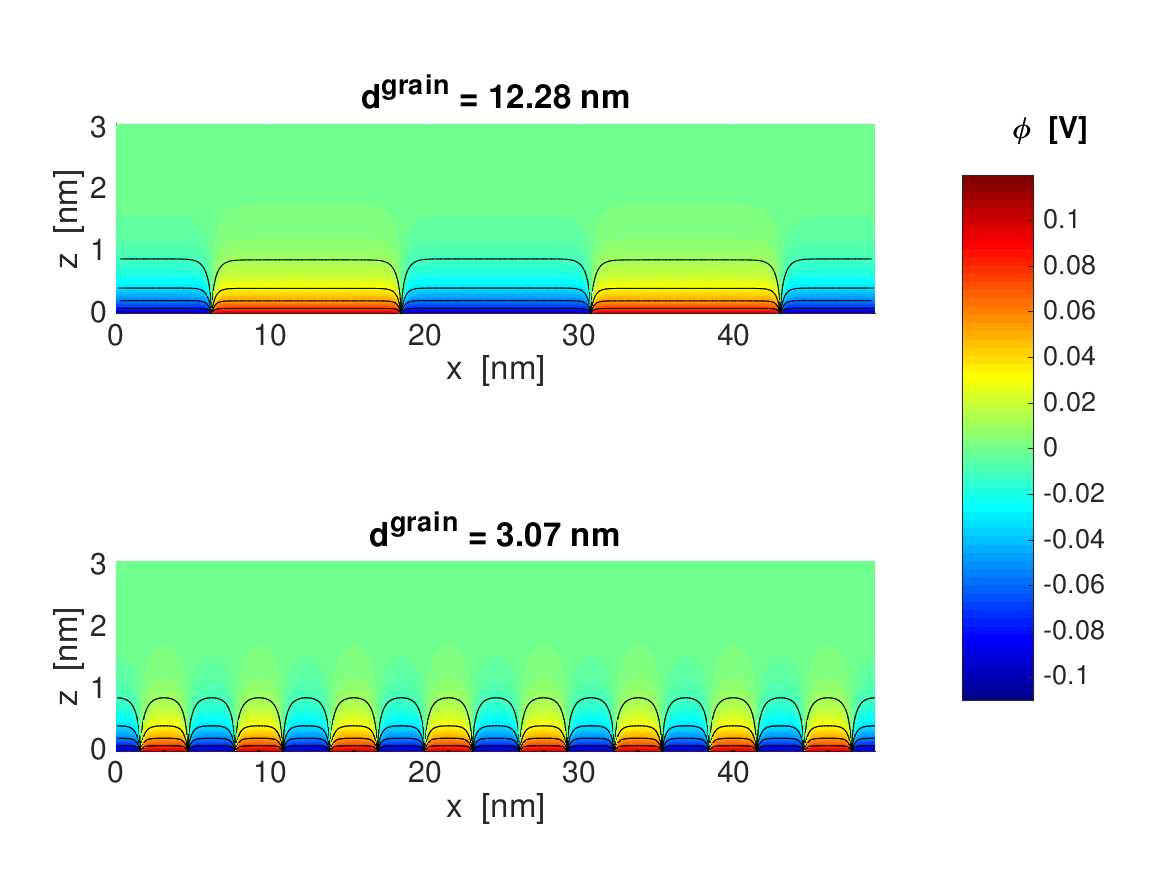
\includegraphics[width=0.45\textwidth]{phi_poly2d_gran.pdf}
  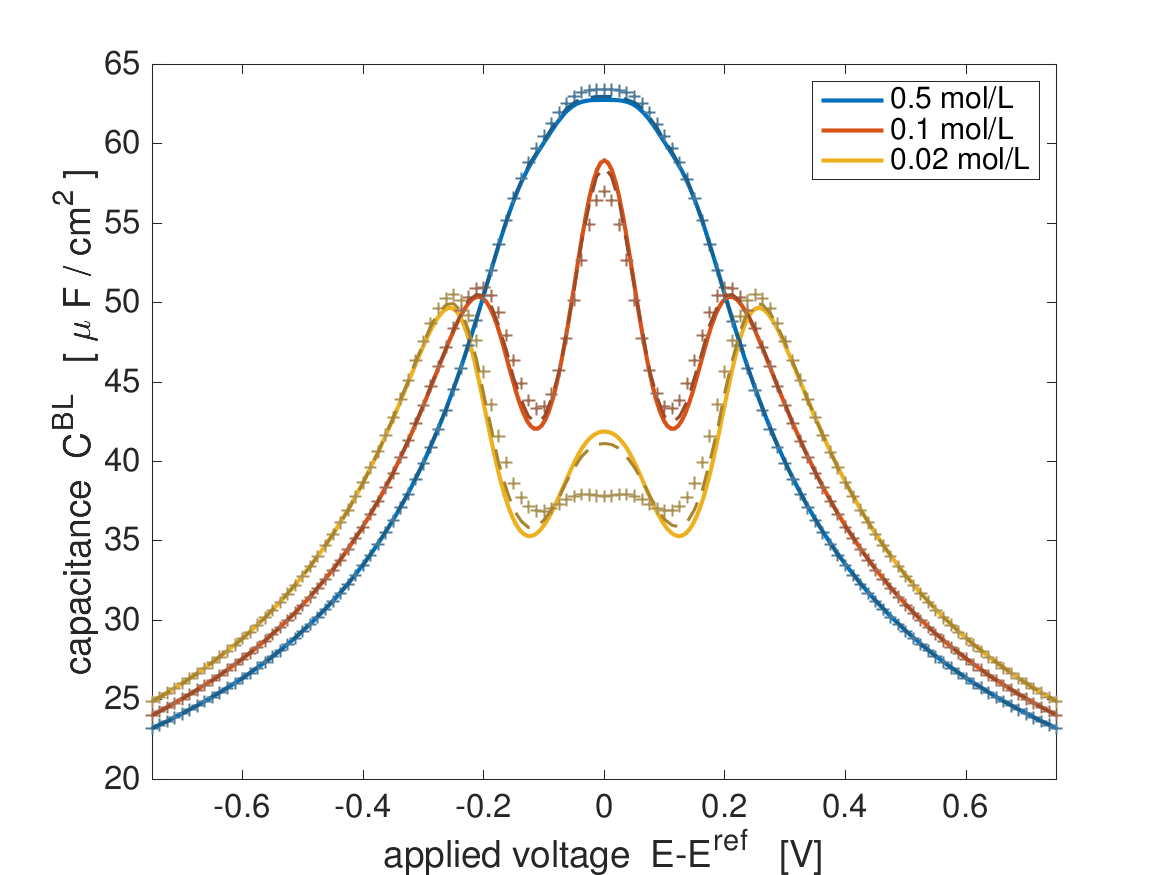
\includegraphics[width=0.45\textwidth]{c_2d_grain.pdf}
  \caption{Left: profile of the electrostatic potential for a bi-crystalline interface with different
    grain sizes.
    Right: double layer capacity curves for different electrolyte concentrations.
    Solid lines (—) refer to the weighted sum of the grain contributions.,
    (+) and dashed (- -) lines mark data obtained from numerical simulations for
    small and large grain sizes, respectively.
 \label{fig:JES}}
\end{figure}




\paragraph{Goals of the Project and Methodologies}
% Please include here:
% - Goals of the project

The results for polycrystalline electrodes  so far are confined to the
case of  thermodynamic equilibrium  and ideally  polarizing electrodes
(without  reactions). They  are an  excellent starting  point for  the
developmennt of  a more general theory  which includes electrochemical
reactions at polycrystalline surfaces. 
In particular, the achieved results provide valuable hints about the most relevant extensions of the modeling framework in order to describe electrocatalytic reactions.
For example the dielectric susceptibility should depend on the local electrolytic concentration
and the temperature. 
Oxide formation on inhomogeneous electrode surfaces can be modeled
by non-monotonous potentials.
The investigation of the dynamics of spatially inhomogeneous reacting surfaces
should lead to effective description of the reactions on a more macroscoptic scale
and extend the stochastic characterization of the polycrystalline electrodes in equilibrium
to the non-equilibrium case.
%
Spatial resolved simulation of the model provides potential surfaces at
some given distance from the electrode surface, essentially corresponding to experimental STM measurements. 
The numerical solution of the transient system allows to simulate CV and to compute the corresponding current--voltage curve. 
This modeling approach is not restricted to CV and STM, but rather the general foundation for the interpretation of 
measurement techniques used in electro-catalysis research as described in the introduction.
%
Accompanied by the development
and implementation  of thermodynamically consistent  numerical methods
and codes, this improved theory of reactive polycrystalline electrodes
shall support  the modeling  of yet  not sufficiently  well understood
features  of experimental  results, with  a possible  outreach to  the
modeling  and simulation  of real  world systems  as described  in the
introduction.
\todo{Dies ist faktisch eine Wiederholung des alten Antrags, der ja
  darauf basierte, dass wir 2 stellen bekommen. Zu seiner Realisierung
  fhelen 36PM Doktorand...}

\todo{Wenn  es komplett neu sein soll:  solar hydrogen - coupling to Perovskites ? -> Koop mit
  LG5, FU, Matera, Unisyscat, HZB, das war auch schon mal für Math+ angedacht.
  RM: das sollte als ein Aspekt dazu}


% - Intended methodologies

The starting point  of the model development is  a general description
for the rate  equations of electrochemical reactions and their coupling to the bulk mass transport
and electrostatic potential at a homogeneous
electrode- electrolyte  interfaces based on the generalized Nernst-Planck-Poisson equations.
To account for non-constant dielectric susceptibility, the structure of the chemical potentials
needs to be extended in a thermodynamically consistent way.
Averaging methods as  developed in
\cite{JES}  are   extended  in   order  provide  rate   equations  for
polycrystalline interfaces  and their respective coupling to the bulk processes.

The modeling process is accompanied by the a numerical implementation based on the
thermodynamically consistent finite volume methods developed in RG3.
On one hand, this implementation will allow to verify the modeling process. On the other
hand the resulting code will be ready to be used in the context of experimental verification.
The development of the numerical schemes will be accompanied by the further investigations
on their thermodynamic consistency and the convergence.

The project can draw on a vast experience with the use of finite volumes schemes for drift-diffusion systems,
as e.g. recent comparison results for different variants of generalized Schafetter-Gummel
schemes, first successful implementations in Julia \cite{VagnerEtAl2019, VoronoiFVM}.
The numerical models will be implemented in  Julia, utilizing forward mode automatic
differentiation to significantly reduce the implementation
effort for strongly nonlinear problems \cite{VoronoiFVM}, reducing the code complexity compared
to C++ and allowing for easy distribution of the code based on a modern package management system.

\paragraph{Main Contributions}
% Please include here BOTH:
% - Impact on mathematics
The project will result in extended bulk-surface models for electrochemical systems which provide
an ample field for further investigation in analysis and numerics. 
Classical electrolyte theory including Debye-H\"uckel theory will be generalized.
Upscaling and averaging methods
for surface rate equations developed in the project are of interest in other applications.

% - Benefit to application area/emerging field
\begin{itemize}
\item Cooperation on modeling and numerics for complex coupled drift-diffusion systems, PDE
  discretization and solution techniques, implementation
\item consistent coupling of electric, thermal and mechanic effects
\end{itemize}


\paragraph{Future Research and New Horizons}
% Please consider the following aspects:
% - Describe the scientific novelties of the project compared to the state-of-the-art in the field of the project.
The establishment of material models for heterogeneously structured electrocatalytically active surfaces
provides the possibility of experimental comparison with polycrystalline or  multi-material electrodes
as they occur in electrochemical experimentation and in real world devices.

% - Highlight the long term research or application perspectives which will be opened by your project.
The ability to model and simulate processes at polycrystalline electrodes will be an excellent foundation
for collaborative research projects in the field of electrochemistry based e.g. on grants available through
the National Hydrogen Initiative.

% - Address potential future research questions / problem complexes which may be approached based on the results upon completion of the project work.
\begin{itemize}
\item Mathematical and numerical  analysis  of the the developed model framework
\item Applications for various different electolyte-interface systems
\end{itemize}
\todo{RM: $\bullet$ optimization of electrocatalytic processes
$\bullet$ improved resolution of STM 
$\bullet$ characterization and identification of real electrode surfaces}

%\nocite{*} % remove this line if you only want to show cited references
\bibliographystyle{mathplusplainyr}
\bibliography{mybibfile}

% This is needed for multiple bib-files
% \printbibliography[heading=none]
% \printbibliography[keyword={reflist},heading=none]

\subsection*{Additional Aspects of the Proposal}

\paragraph{Collaborations}
% Please list existing or planned cooperation (scientific, industrial, ...),
% both internal and external. Sort as follows:
% - Internal cooperation (within MATH+)
\begin{itemize}
\item Glitzky ...
\item Farrell ...
\item weiteres noch zu klären
\end{itemize}

% - External scientific cooperation (outside MATH+)
\begin{itemize}
\item Fortschreibung der Kooeprationen aus dem alten Antrag ?
\end{itemize}
% - External industrial cooperation (outside MATH+)

\paragraph{Related Projects}
% Please include your funded projects which are topicwise related to this proposal.
% State the main differences.
\begin{itemize}
\item EDLSOC: solid electorlytes, non-isothermal
\item LuCaMag: not focused on multi-material
\item Malli2: 
\end{itemize}

\paragraph{Further Impact of the Project on MATH$+$}
% Please discuss different types of impact of your project on
% MATH+. Sort as follows:
% - Additional Funding (Further funding of research themes related to this project)
We see a good perspective for additional funding based on the modeling and simulation approach
developed in this project.

% - Research Training (Summer schools, etc.)
Results and approached from the project will be used in the 

% - Gender and Diversity (Activities for female students, etc.)
We will participate education of a diverse group of people in the teaching activities

% - Complementary Skills (Opportunities for project staff to acquire skills complementing existing ones)
Obtain further skills in numerical methods and their implementation, unique skills in electrochemical
modeling asked for in  industry

% - Outreach (Plenary lectures, public lectures, etc.)
We will participate in public outreach activities

\paragraph{Position(s) of the PI(s)}
% It is required that the position(s) of all PIs is/are secured for the complete duration of the project applied for. PIs on a fixed-term contract should provide corresponding evidence through a statement by their supervisor (e.g. project proposal XY currently being reviewed/extended by third party funding agency ZZ). 
% Junior-Profs and Junior Research Group Leaders should refer to the envisioned date of their interim evaluation. 
Both PIs have tenure positions at Weierstrass Institute.

\end{document}

